\section{Crowd plug-in}

The goal of this work package was to implement an efficient and realistic motion of a crowd. \\
The initial goal was to implement two parts: one creating trajectories for the crowd and another one for animating individual movements. The second part was really hard to implement and had a lot of relation with animation of models, in which we don't know anything. Thus we decided to concentrate ourselves on the first part.\\
Our code is split into two parts: one that is independent from Blender and one that depends on it (see figure \ref{fig:code}). \\
The first part create a set of key points that will represent the movement of one person and the second interpolate a trajectory from those points.


\subsubsection{Human animation}

At the beginning we considered animating Humans and started by analyzing a theoretical survey of Computer animation of Human walking (\cite{th_walking}) and looking for what was already done in Blender concerning automatic walking. All Blender-related resources on walking animation are gathered on a web-page (\cite{blwikiwalking}). Walk-o-matic and stride add-ons were used in previous versions of Blender to ``help to interactively design rough passes of a walk'' and ``quickly create cycles for background or extra characters'', however both were broken on Blender 2.7 and we are using Blender 2.76. 

Due to the lack of existing tools concerning automatic walking we considered creating such a tool ourselves. We started by analyzing tutorials on blender character animation (for example \cite{tuto_walk}) and creating such a motion manually. However we soon realized how difficult it is to generate a realistic walk due to the complex physics behind the movements and decided that it is out of the scope of our project. We have shifted our attention to the more basic task of creating a path in Blender and making an object following it with varying speed given by our algorithm.


% Il faudra changer les titres je pense 
\subsection{Algorithm description}

The first algorithm is inspired by those two papers: \cite{PLE} and \cite{vandenBerg2011}. We chose them because the notions involved in the description of the algorithm were more familiar to us.
% TODO : combler avec du bla bla
The idea is the following: a graph (grid) algorithm will generate a general path for each individual and another algorithm will prevent collisions between individuals. \\
Time is discretized, and for each time, we compute the direction to go for each individual. We move the in this direction, and iterate this principle. This is how we get the final set of points for each individuals.


\subsection{Algorithm implementation}

\subsubsection{The guide graph}

The first part that we tried to implement was the data structure of the graph. We created a data structure representing the nodes of the graph and the edges. This was quite easy to do since the graph is supposed to be a grid, it is regular.
Then we needed a minimum distance (1 to 1) algorithm on the graph. For that we chose the $A^*$ algorithm. Unfortunately, our implementation of the $A^*$ was really costly in time and even more in memory. This fact forced us to abandon the graph in the rest of the development. We could test it for small values, and for a small number of calls, but the $A^*$ procedure would have to be called thousands of times which makes this impractical. 
To replace the graph we used the euclidean distance, this involved removing statics obstacles. Also the points were no more able to avoid packed places and just went strait to there goal.

\subsubsection{Allowed velocity field}

This part deals with collision avoidance. This part is the part that took us the more time to implement. The problem is the following, you have a set of individual (i.e. points) with current velocities. You want for each individual a set of velocities that will ensure that  if we pick one in it then we will not collide with another individual on the way. To do that the algorithm makes a lot of geometrical computation as explained in \cite{vandenBerg2011}. We used the python library Shapely to represent geometrical structures. 

%% WHat kind of errors ?
This library has some very useful tools but some functionalities did not work very well with floating-point numbers and the small approximations that they entail. The errors linked to the floats are one of the main reason it took us time. %% TO WHAT ?
The other was that some geometrical forms were hard to represent and to compute both theoretically and computationally.
Also due to the absence of the guide graph, the individuals were not able to go around ob stables so it induced bugs, the points tends to get closer and closer to the limits of the obstacle until they cross it through errors and thus go through obstacles.
In the end, this part does return collisions free velocities in 95\% of cases. There are still some bugs that we were not able to find.
%% Figure du beamer ?
%% Bugs not able to find ? to resolve ?

\subsubsection{Computation of the allowed movement}

This part involves minimizing a function on the velocity field of each individuals. For that we had two options. The first one was to implement a simplex but the graph was not a linear constraint so we thought that this was not a valid way to minimize.
%% Lien avec le graphe ?
 The second method was to choose an angle and increment it according to a $d\theta$ and minimizing the function on those angles.
%% Quelle fonction ?
This part is fully functional but relied on floating-point numbers again, involving computational errors.


\subsection{Path generation in Blender}

The algorithm described in the previous paragraphs outputs individual's coordinates at every time step and from these we have to interpolate a continuous path in Blender. 


\subsubsection{Creating a path}

There are two ways to make an object move in Blender
\begin{enumerate}
\item Fix where an object should be at a given time and then modify the interpolation of the movement to make it realistic.  
\item Use Blender structures for paths (Bezier curves, NURBS curves) and various ways to couple an object and a path (\textit{Follow Path} Constraint, \textit{Clamp To} Constraint).
\end{enumerate} 

All of these options generate movement, however our work was to find the one that could be automated easily, that would be compatible with a data structure given by our algorithm, that would be precise and easy to modify for the user afterwards. 

The first option was compatible with our data structure however realistic interpolation of the path and possibility to modify a path afterwards posed us a lot of questions and we have chosen the second option which is a more conventional one, makes a clear distinction between a path and an object following it and is easy to modify for an artist afterwards. 

The main problem to solve was a discrepancy between the data structures: position of an object on the path (Bezier or NURBS) is given through its distance along the path from the starting point while in the data structure given by our algorithm position of the point is accessed through its coordinates \textcolor{red}{(ça ça montre pas un manque flagrant de coordination?)}. This being said we had to find a way to link a position in the space to the length of the path from the starting point to that position. Blender 2.76 having no add-on to measure the length of the path made this task more complicated as we had to familiarize with the mathematics behind the interpolation of Bezier curves and NURBS.   

We have chosen Bezier curves instead of NURBS because their mathematical properties allowed us to guarantee that an individual will be at a given place at a given time while NURBS interpolates a path that only comes close to the given points but not necessary passes through them.

\subsection{GUI}
The approach we chose was to have a GUI that would be integrated in the Blender GUI.\\
There where many layers of GUI in Blender:
\begin{itemize}
\item window
\item banner
\item pannel
\end{itemize}

We chose to make panels for simplicity reasons and we put those in the right banner of the 3DVIEW window.\\
Once we mastered the making and integrating of panels with simple functionalities in Blender we started to separate the functionalities we wanted for the GUI of the crowd plug-in.

\subsubsection{The Map Panel}
The first panel we decided to create was one to create the map and grid on which the crowd will evolve.\\
We created it with four main functionalities:
\begin{itemize}
\item save and load the current map
\item adjust size and origin of the map
\item adjust grid size (crucial for the algorithm)
\item add exclusion zones
\end{itemize}


\subsubsection{The Crowd Panel}
The second panel provides three of methods to create a crowd 
\begin{itemize}
\item save and load
\item initialisation with default settings
\item initialisation with random settings
\end{itemize}

We also chose to add a personalization feature: from an existing crowd (initialized with one of the three methods above) the user can select an individual and change all of its settings: initial position, goal, size, optimal speed, maximal speed and animation of the individual.


\subsubsection{The Simulation Panel}
The last panel allows the user to launch the computation of a crowd animation and to render it in Blender.\\
The user must first set the time quantum, number of time quantum to be computed and angle quantum and then the user can launch computation and load the resulting animation into Blender's 3DVIEW.\\
There is also a save and load functionality for the animation.

\begin{figure}
  \centering
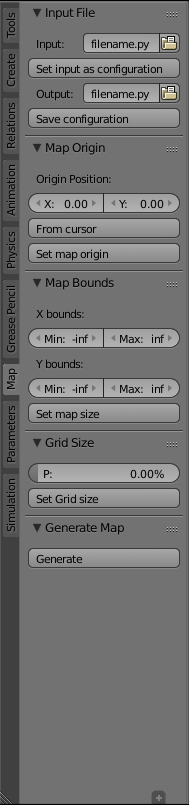
\includegraphics[height=10cm]{img/GUI_map_example.png} ~ 
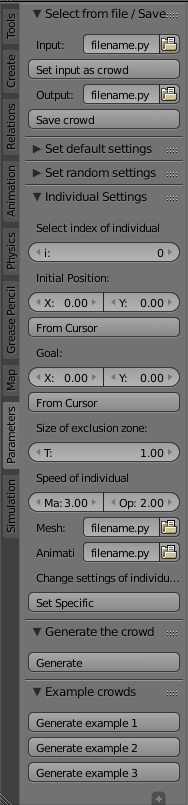
\includegraphics[height=10cm]{img/GUI_crowd_example.png} ~ 
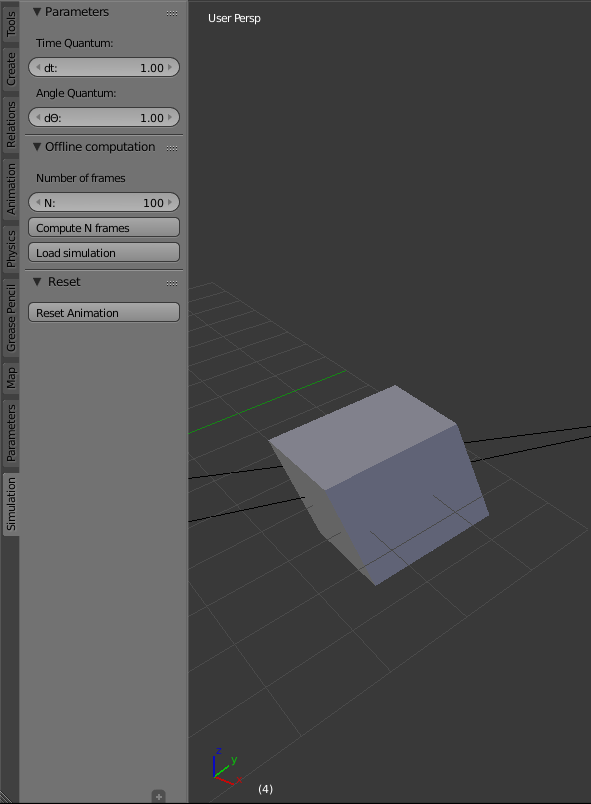
\includegraphics[height=10cm]{img/GUI_simulation_example.png}
\end{figure}
